Nel caso precedente è stato automaticamente posto nullo il 
campo di spostamento elettrico all'esterno del condensatore, per
dimostrare ciò si suppone di avere uno strato piano di carica libera indefinito:
\begin{figure}[H]
\centering
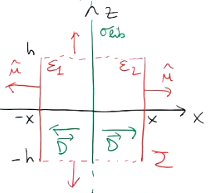
\includegraphics[width=0.3\linewidth]{lastra_piana_dielettrico}
\caption{Lastra piana carica}
\end{figure}
I due semipiani avranno costanti dielettriche differenti $\varepsilon_1$ 
ed $\varepsilon_2$.
Si studia il campo utilizzando la legge di Gauss:
$$
\oiint_{\Sigma} \vec{D}\cdot\hat{n}dS = Q_{lib}
$$
In questo caso si prende un parallelepipedo parallelo alle facce. La 
simmetria della distribuzione rispetto agli assi $y$ e $z$ fanno sì
che $\vec{D} = D_x(x)\vec{e}_x$ (in seguito $D_x$ sarà semplicemente $D$).

Applicando la legge di Gauss alla superficie $\Sigma$ si evince subito
che le superfici ortogonali ad $x$ non contribuiscono al flusso.
$$
\frac{\oiint_\Sigma \vec{D} \cdot \hat{n} dS }{hL}= -2\cancel{hL} D(-x) + 2\cancel{hL}D(x) = 
\sigma_{lib}\cancel{hL}
$$
Si evince la simmetria dispari del campo rispetto alla coordinata $x$ 
ossia $D(-x) = -D(x)$, sostituendo nella precedente si ottiene
$$
2D(x) = \sigma_{lib} \Rightarrow D(x) = \frac{\sigma_{lib}}{2}
$$
Il campo $\vec{D}$ è quindi pari in modulo e diretto in versi opposti
nei due semipiani. Per calcolare il campo $\vec{E}$ si potrà usare
la relazione costitutiva
$$
\vec{E} = \frac{\vec{D}}{\varepsilon}\Rightarrow
\begin{cases}
x > 0, & \vec{E}=\frac{\sigma_{lib}}{2\varepsilon_2} \vec{e}_x \\
x < 0, & \vec{E} = -\frac{\sigma_{lib}}{2\varepsilon_1} \vec{e}_x
\end{cases}\qquad
\begin{aligned}
\hat{n}\cdot(\vec{D}_2-\vec{D}_1) &= \sigma_{lib}\\
\hat{n}\cdot (\vec{E}_2-\vec{E}_1) &= \frac{\sigma_{lib}+\sigma_{pol}}{\varepsilon_0}
\end{aligned}
$$
Vale la continuità della componente normale di $\vec{D}$ ed $\vec{E}$.

\subsection{Condensatore piano con dielettrico}
Utilizzando il PSE, si prendono due strati indefiniti di carica $-\sigma_{lib}$ e $\sigma_{lib}$ mentre all'ascissa $x_0$ si trova un
cambio di dielettrico, come rappresentato in figura
\begin{figure}[H]
\centering
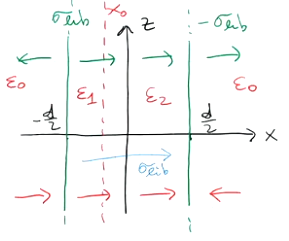
\includegraphics[width = 0.4\linewidth]{condensatore_dielettrici}
\caption{Lastre piane indefinite con dielettrici}
\end{figure}
Il campo $\vec{D}$ prodotto dall'armatura carica di sinistra sarà un campo uniforme
e diretto in verso uscente dalla lastra. Viceversa il campo prodotto
dalla lastra di destra sarà entrante nella lastra a causa del segno
opposto della carica.

La sovrapposizione degli effetti permette di calcolare il campo
totale eseguendo la somma dei due, all'esterno delle armature
il campo sarà quindi nullo mentre all'interno sarà di valore pari
a $\sigma_{lib}$
$$
\vec{D}(x) = \begin{cases}
\sigma_{lib} \vec{e}_x, & |x|<\frac{d}{2}\\
0 & \text{altrimenti}
\end{cases}
$$
È ora necessario calcolare il campo $\vec{E}$ e la capacità del 
condensatore, utilizzando i differenti valori di $\varepsilon$:
$$
\varepsilon = \begin{cases}
\varepsilon_0, & x< -\frac{d}{2}\\
\varepsilon_1, & -\frac{d}{2} < x < x_0 \\
\varepsilon_2, & x_0 < x < \frac{d}{2}\\
\varepsilon_0, & x>\frac{d}{2}
\end{cases}
$$
Sfruttando le relazioni costitutive si può ora calcolare
il campo $\vec{E}$
$$
E(x) = \begin{cases}
0, & x < -\frac{d}{2} \\
\frac{\sigma_{lib}}{\varepsilon_1}, & -\frac{d}{2} < x < x_0\\
\frac{\sigma_{lib}}{\varepsilon_2}, & x_0 < x < \frac{d}{2}\\
0, & x > \frac{d}{2}
\end{cases}
$$
Per calcolare la differenza di potenziale è sufficiente calcolare la 
differenza tra la funzione potenziale all'ascissa $-\frac{d}{2}$ e un 
punto $x$ generico
\begin{align*}
&V\left(-\frac{d}{2}\right) - V(x) = \int_{-\frac{d}{2}}^{x} \frac{\sigma_{lib}}{\varepsilon_1} d\xi = \frac{\sigma_{lib}}{\varepsilon_1}\left(x+\frac{d}{2}\right), -\frac{d}{2} < x < x_0 \Rightarrow V(x) = V^+ - \frac{\sigma_{lib}}{\varepsilon_1}\left(x + \frac{d}{2}\right)\\
&V(x_0 )- V(x) = \int_{x_0}^{x} \frac{\sigma_{lib}}{\varepsilon_2} d\xi = \frac{\sigma_{lib}}{\varepsilon_2} (x-x_0), x_0<x<\frac{d}{2}  \Rightarrow V(x) = V^+ - \frac{\sigma_{lib}}{\varepsilon_1}\left(x_0+\frac{d}{2}\right) - \frac{\sigma_{lib}}{\varepsilon_2}(x-x_0)
\end{align*}
Eseguendo quindi la differenza tra i potenziali sulle due armature si ottiene:
$$
V\left(-\frac{d}{2}\right) - V\left(\frac{d}{2}\right) = \cancel{V^+} - \left[ \cancel{V^+} -\frac{\sigma_{lib}}{\varepsilon_1}\left(x_0+\frac{d}{2}\right) - \frac{\sigma_{lib}}{\varepsilon_2} (x-x_0)\right] = \sigma_{lib} \left[\frac{1}{\varepsilon_1}\left(x_0+\frac{d}{2}\right) + \frac{1}{\varepsilon_2}\left(\frac{d}{2}-x_0\right)\right]
$$

La capacità sarà quindi 
$$
C = \frac{Q_{lib}}{V\left(-\frac{d}{2}\right) - V\left(\frac{d}{2}\right)} = 
\frac{\cancel{\sigma_{lib}}S}{\cancel{\sigma_{lib}} \left[ \frac{1}{\varepsilon_1}\left(x_0+\frac{d}{2}\right) + \frac{1}{\varepsilon_2}\left(\frac{d}{2}-x_0\right) \right] }
$$
Semplificando:
\begin{equation}
C = \frac{1}{ \frac{1}{\varepsilon_1S} \left(x_0 + \frac{d}{2} \right) + \frac{1}{\varepsilon_2S} \left( \frac{d}{2} - x_0 \right) } = \frac{1}{\frac{1}{C_1}+\frac{1}{C_2}}
\label{eq:condensatore_dielettrico}
\end{equation}
Nel condensatore vuoto la capacità era
$$
C_{\text{vuoto}} = \varepsilon_0\frac{S}{d}
$$
Si nota quindi che al denominatore della \ref{eq:condensatore_dielettrico} c'è la somma di due
reciproci di capacità $\frac{1}{C_1}$ e $\frac{1}{C_2}$ dove $C_1$ e $C_2$ sono appunto
$$
C_1 = \varepsilon_1 \frac{S}{x_0 + \frac{d}{2}} \qquad C_2 = \varepsilon_2 \frac{S}{\frac{d}{2}-x_0}
$$
Si vede quindi che la formula ottenuta è identica a quella di due condensatori in serie,
il primo di spessore $x_0 + \frac{d}{2}$ e il secondo $\frac{d}{2}-x_0$ adiacenti sulla faccia
$x_0$ e ciascuno con la propria costante dielettrica.

Lo stesso risultato si sarebbe potuto ottenere utilizzando il \textit{principio di metallizzazione delle 
superfici equipotenziali}.

Siccome la funzione potenziale è anch'essa funzione della sola coordinata $x$,  le superfici 
equipotenziali sono del tipo $x=a$, qualunque piano perpendicolare all'asse $x$ è una superficie
equipotenziale.

In virtù dell'unicità dei problemi dei valori al contorno dell'equazione di Laplace (o Poisson)
si può sostituire alla superficie di interfaccia tra i dielettrici, nel punto $x_0$ un conduttore
metallico stratiforme.
Fatto ciò è evidente vedere i due condensatori, la superficie metallica funge proprio
da armatura per entrambi i condensatori, disposti in serie.
\newpage
\subsection{Richiami su condensatori in serie e in parallelo}
\paragraph{Sistema serie}
\begin{figure}[H]
\centering
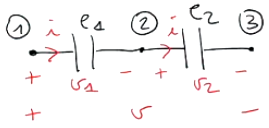
\includegraphics[width = 0.3\linewidth]{condensatori_serie}
\end{figure}
Presi due condensatori $C_1$ e $C_2$ disposti in serie, saranno attraversati dalla stessa corrente
$i$ e nel circuito saranno presenti tre potenziali sui nodi (1), (2) e (3).

Le equazioni caratteristiche sono:
\begin{align*}
&i = C_1 \frac{dv_1}{dt}\\
&v_1(t_0) = V_{10}\\
&i = C_2 \frac{dv_2}{dt} \\
&v_2(t_0) = V_{20}
\end{align*}
\begin{align}
v(t) = v_1(t) + v_2(t)
\label{eq:relazione_serie}
\end{align}
Integrando la prima e la terza relazione tra $t_0$ e $t$ si ottiene
\begin{align*}
&\int_{t_0}^t i(\tau) d\tau = C_1 \left[v_1(t) - V_{10}\right] \\
&\int_{t_0}^t i(\tau)d\tau = C_2 \left[v_2(t) - V_{20}\right]
\end{align*}
e sottraendo membro a membro
$$
C_1 \left[v_1(t) -V_{10}\right] = C_2\left[v_2(t) - V_{20}\right]
$$
Ricaviamo $v_2$ dalla precedente
$$
v_2(t) = V_{20} + \frac{C_1}{C_2} \left[v_1(t) - V_{10} \right]
$$
Utilizzando la relazione \ref{eq:relazione_serie} e sostituendo $v_2$ si ottiene
$$
v_1(t) = v(t) - V_{20} - \frac{C_1}{C_2} \left[v_1(t) - V_{10}\right]
$$
$$
v_1(t)\left(1+\frac{C_1}{C_2}\right) = v(t) - V_{20} + V_{10}\frac{C_1}{C_2}
$$
$$
v_1(t) = \frac{C_2}{C_1+C_2} v(t) + \frac{C_2}{C_1+C_2}\left[\frac{C_1}{C_2}V_{10}-V_{20}\right]
$$
$$
v_2(t) = \frac{C_1}{C_1+C_2} v(t) + \frac{C_1}{C_1+C_2}\left[\frac{C_2}{C_1}V_{20}-V_{10}\right]
$$
Sostituendo l'equazione di $v_1(t)$ nella caratteristica $i = C_1\frac{dv_1}{dt}$ si 
ottiene 
$$
i = \frac{C_1C_2}{C_1+C_2}\frac{dv}{dt}
$$
dato che il secondo termine di $v_1(t)$ è costante e la sua derivata è nulla. Il 
coefficiente ottenuto è proprio la capacità equivalente della serie.

\paragraph{Condensatori in parallelo}
\begin{figure}[H]
\centering
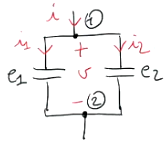
\includegraphics[width = 0.3\linewidth]{condensatori_parallelo}
\end{figure}

I due condensatori sono sottoposti alla stessa tensione $v$ ma attraversati da due
differenti correnti.
\begin{align*}
&i_1 = C_1 \frac{dv}{dt} \\
& i _2 = C_2 \frac{dv}{dt} \\
& v(t_0) = V_0
\end{align*}
In questo caso, a differenza del precedente si ha una sola grandezza di stato.
Sfruttando la legge di Kirchhoff delle correnti al nodo (1) si ottiene
$$
i = i_1 + i_2 = (C_1+C_2) \frac{dv}{dt}
$$
quindi
$$
\frac{dv}{dt} = \frac{i}{C_{eq}} \Rightarrow \begin{cases}
i_1 = \frac{C_1}{C_{eq}}i = \frac{C_1}{C_1+C_2}i\\
i_2 = \frac{C_2}{C_{eq}}i = \frac{C_2}{C_1 + C_2}i
\end{cases}
$$

\subsection{BVP per condensatore a due dielettrici}
\begin{figure}[H]
\centering
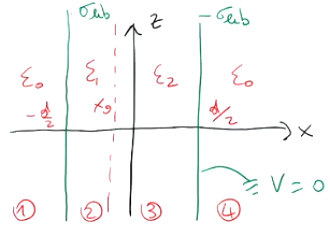
\includegraphics[width = 0.3\linewidth]{condensatore_dielettrici_2}
\end{figure}
Rappresentiamo graficamente il condensatore, applichiamo le equazioni
di Laplace alle diverse regioni
\begin{align*}
\nabla^2 V_1 = 0 \qquad & x< -\frac{d}{2} & V_1(x) = Ax + B\\
\nabla^2 V_2 = 0 \qquad & -\frac{d}{2} < x < x_0 & V_2(x) = Cx + D\\
\nabla^2 V_3 = 0 \qquad & x_0 < x < \frac{d}{2} & V_3(x) = Ex + F \\
\nabla^2 V_4 = 0 \qquad & x > \frac{d}{2} & V_4(x) = Gx + H
\end{align*}
Ricordando che in un problema monodimensionale
$$
\nabla^2 V = \frac{d^2 V}{dx^2} = 0 \Rightarrow V(x) = k_1x + k_2
$$
Si impostano due costanti per ogni regione, per un totale di 8
determinabili mediante le condizioni al contorno e di raccordo.

Le condizioni sono:
\begin{align*}
1) \qquad &V_1\left(-\frac{d}{2}\right) = V_2\left(-\frac{d}{2}\right)\\
2) \qquad &V_2\left(x_0\right) = V_3\left(x_0\right)\\
3) \qquad &V_3\left(\frac{d}{2}\right) = V_4\left(\frac{d}{2}\right)\\
4) \qquad  &
-\varepsilon_1 \left.\frac{\partial V_2}{\partial x}\right|_{-\frac{d}{2}} +
\varepsilon_0 \left.\frac{\partial V_1}{\partial x}\right|_{-\frac{d}{2}} = 
\sigma_{lib}\\
5) \qquad &-\varepsilon_2 \left.\frac{\partial V_3}{\partial x}\right|_{x_0} +
\varepsilon_1 \left.\frac{\partial V_2}{\partial x}\right|_{x_0} = 
0\\
6) \qquad &-\varepsilon_0 \left.\frac{\partial V_4}{\partial x}\right|_{\frac{d}{2}} +
\varepsilon_2 \left.\frac{\partial V_3}{\partial x}\right|_{\frac{d}{2}} = 
-\sigma_{lib}\\
7) \qquad &V_3\left(\frac{d}{2}\right) = 0 \qquad \text{pot. di riferimento}\\
8-9) \qquad& -\frac{\partial V_1}{\partial x} ,\ -\frac{\partial V_4}{\partial x} = 0\ \ |x| > \frac{d}{2}\ \ \text{campo esterno nullo}
\end{align*}
Il potenziale di riferimento è necessario dato che essendo le superfici cariche 
infinite, non si ha un potenziale normale all'infinito, questo
viola il teorema di unicità della soluzione rendendo necessario il riferimento.
Non conta il valore di riferimento assegnato dato che la grandezza di interesse
è il campo elettrico, ossia il gradiente del potenziale che non dipende
dal suo riferimento.

L'ultima condizione (8-9) deriva dall'estensione all'infinito dei modelli al 
finito che prevedono un campo elettrico concentrato al centro. Anche i modelli
all'infinito devono rispettare quindi la normalità all'infinito, ossia il
campo deve essere nullo al di fuori delle armature.

Riscrivendo le equazioni con le costanti incognite si ottiene:
\begin{align*}
1)   \qquad & A\left(-\frac{d}{2}\right) + B = C\left(-\frac{d}{2}\right) + D \\
2)   \qquad & Cx_0 + D = Ex_0 + F \\
3)   \qquad &E\frac{d}{2} + F = G \frac{d}{2} + H \\
4)   \qquad &- \varepsilon_1 C + \varepsilon_0 A = \sigma_{lib} \\
5)   \qquad &- \varepsilon_2 E + \varepsilon_1 C = 0 \\
6)   \qquad &-\varepsilon_0G = \varepsilon_2 E = -\sigma_{lib} \\
7)   \qquad & E\frac{d}{2} + F = 0 \\
8-9) \qquad & A = G = 0
\end{align*}

Ci sono quindi 9 equazioni in 8 incognite e si può vedere che il sistema 
ha rango 8.
Si può porre il sistema lineare con notazione matriciale nel seguente modo:
\begin{align*}
\underline{\underline{A}}\ \underline{x} &= \underline{b}\\
\underline{x} &= \left(A,B,C,D,E,F,G\right)^T \\
\underline{b} &= \left(0,0,0,\sigma_{lib},0,-\sigma_{lib},0,0\right)^T 
\end{align*}
Mentre la matrice $\underline{\underline{A}}$ si deduce dall'analisi delle 
equazioni. 
\newpage
Di seguito è riportato un esempio per risolvere numericamente
il problema.
\begin{lstlisting}[style=Matlab-editor,language = Matlab]
syms d Vp x0 ep0 ep1 ep2 slib x real

A = [ -d/2   1   d/2   -1   0   0   0   0;
        0    0    x0    1  -x0 -1   0   0;
        0    0    0     0  d/2  1 -d/2 -1;
       ep0   0  -ep1    0   0   0   0   0;
        0    0   ep1    0 -ep2  0   0   0;
        0    0    0     0  ep2  0 -ep0  0;
        0    0    0     0  d/2  1   0   0;
        1    0    0     0   0   0   0   0;
        0    0    0     0   0   0   1   0];

b=[0;0;0;slib;0;-slib;0;0;0];

K=A\b; %Vettore delle costanti incognite
V1=K(1)*x+K(2);
V2=K(3)*x+K(4);
V3=K(5)*x+K(6);
V4=K(7)*x+K(8);

V=[V1;V2;V3;V4]
E=-diff(V,x)
D=diag([ep0,ep1,ep2,ep0])*E
\end{lstlisting}
1:27:58

